
\documentclass[12pt,letterpaper]{article}
\usepackage{graphicx,textcomp}
\usepackage{natbib}
\usepackage{setspace}
\usepackage{fullpage}
\usepackage{color}
\usepackage[reqno]{amsmath}
\usepackage{amsthm}
\usepackage{fancyvrb}
\usepackage{amssymb,enumerate}
\usepackage[all]{xy}
\usepackage{endnotes}
\usepackage{lscape}
\newtheorem{com}{Comment}
\usepackage{float}
\usepackage{hyperref}
\newtheorem{lem} {Lemma}
\newtheorem{prop}{Proposition}
\newtheorem{thm}{Theorem}
\newtheorem{defn}{Definition}
\newtheorem{cor}{Corollary}
\newtheorem{obs}{Observation}
\usepackage[compact]{titlesec}
\usepackage{dcolumn}
\usepackage{tikz}
\usetikzlibrary{arrows}
\usepackage{multirow}
\usepackage{xcolor}
\newcolumntype{.}{D{.}{.}{-1}}
\newcolumntype{d}[1]{D{.}{.}{#1}}
\definecolor{light-gray}{gray}{0.65}
\usepackage{url}
\usepackage{listings}
\usepackage{color}
\usepackage{hyperref}

\definecolor{codegreen}{rgb}{0,0.6,0}
\definecolor{codegray}{rgb}{0.5,0.5,0.5}
\definecolor{codepurple}{rgb}{0.58,0,0.82}
\definecolor{backcolour}{rgb}{0.95,0.95,0.92}

\lstdefinestyle{mystyle}{
	backgroundcolor=\color{backcolour},   
	commentstyle=\color{codegreen},
	keywordstyle=\color{magenta},
	numberstyle=\tiny\color{codegray},
	stringstyle=\color{codepurple},
	basicstyle=\footnotesize,
	breakatwhitespace=false,         
	breaklines=true,                 
	captionpos=b,                    
	keepspaces=true,                 
	numbers=left,                    
	numbersep=5pt,                  
	showspaces=false,                
	showstringspaces=false,
	showtabs=false,                  
	tabsize=2
}
\lstset{style=mystyle}
\newcommand{\Sref}[1]{Section~\ref{#1}}
\newtheorem{hyp}{Hypothesis}

\title{Problem Set 1}
\date{Maiia Skrypnyk 23371609}
\author{Applied Statistical Analysis 1}

\begin{document}
	\maketitle

	\section*{Question 1 (40 points): Education}

A school counselor was curious about the average of IQ of the students in her school and took a random sample of 25 students' IQ scores. The following is the data set:\\

\lstinputlisting[language=R, firstline=39, lastline=39]{PS01MS.R}  
\vspace{.5cm}

\begin{enumerate}
	\item Find a 90\% confidence interval for the average student IQ in the school.

\lstinputlisting[language=R, firstline=45, lastline=100]{PS01MS.R}  
\vspace{.2cm}

	\item Next, the school counselor was curious  whether  the average student IQ in her school is higher than the average IQ score (100) among all the schools in the country.\\ 
	
	\noindent Using the same sample, conduct the appropriate hypothesis test with $\alpha=0.05$.
	
	\lstinputlisting[language=R, firstline=108, lastline=150]{PS01MS.R}  
	\vspace{.2cm}
\end{enumerate}

\newpage

	\section*{Question 2 (40 points): Political Economy}

\noindent Researchers are curious about what affects the amount of money communities spend on addressing homelessness. The following variables constitute our data set about social welfare expenditures in the USA. \\
\vspace{.5cm}


\begin{tabular}{r|l}
	\texttt{State} &\emph{50 states in US} \\
	\texttt{Y} & \emph{per capita expenditure on shelters/housing assistance in state}\\
	\texttt{X1} &\emph{per capita personal income in state} \\
	\texttt{X2} &  \emph{Number of residents per 100,000 that are "financially insecure" in state}\\
	\texttt{X3} &  \emph{Number of people per thousand residing in urban areas in state} \\
	\texttt{Region} &  \emph{1=Northeast, 2= North Central, 3= South, 4=West} \\
\end{tabular}

\vspace{.5cm}
\noindent Explore the \texttt{expenditure} data set and import data into \texttt{R}.
\vspace{.5cm}
\lstinputlisting[language=R, firstline=172, lastline=172]{PS01MS.R}  
\begin{itemize}

\item
\textbf {Please plot the relationships among \emph{Y}, \emph{X1}, \emph{X2}, and \emph{X3}? What are the correlations among them (you just need to describe the graph and the relationships among them)?}
\vspace{.2cm}
\end{itemize}

\noindent \begin{center}
	\textbf {\textit{2.1.1:YX1}}
\end{center}

\noindent \begin{center}
	\textit{(Please see the plot on the next page)}
\end{center}


\begin{figure}[H]
	\centering
	\caption{\footnotesize Relationship between Per capita state expenditure and Per capita personal income}
	\label{fig:plot_1}
	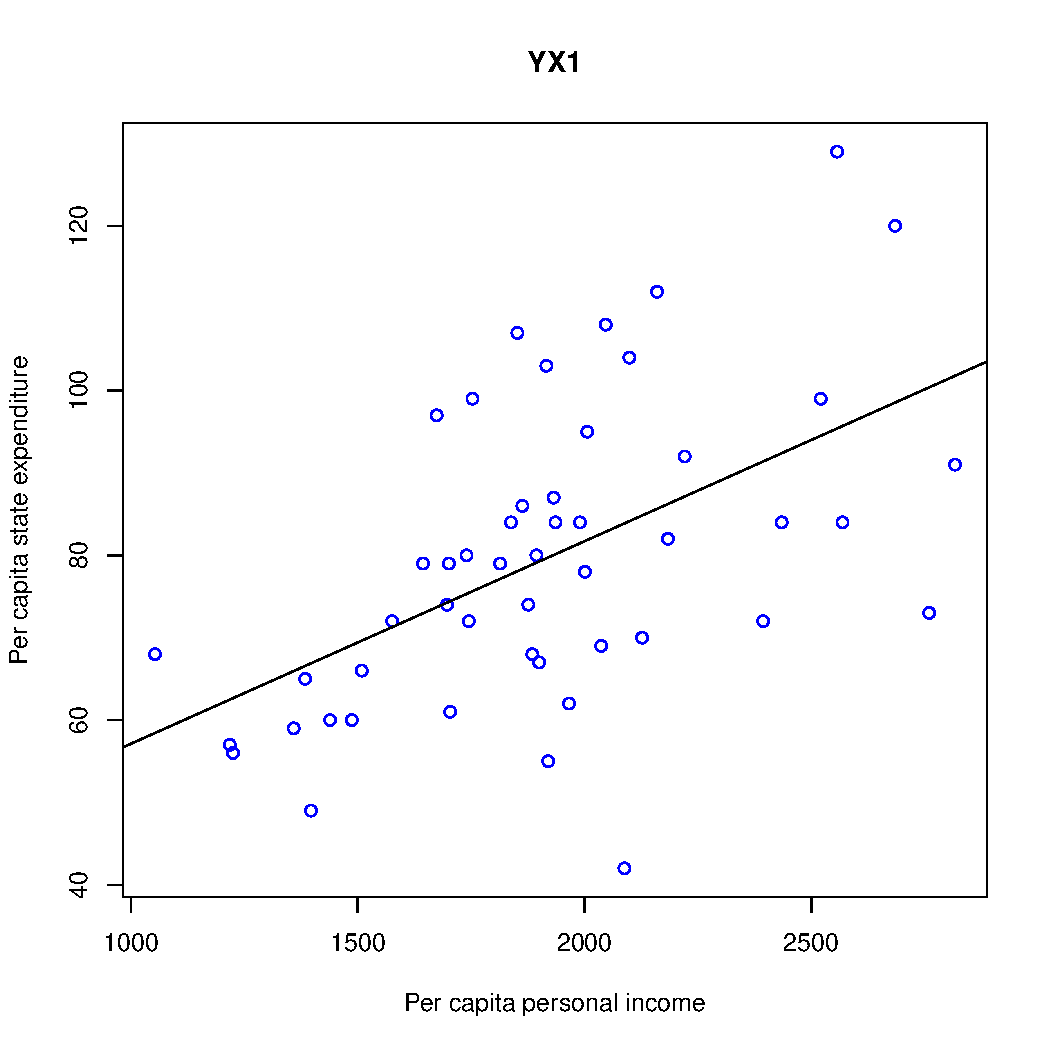
\includegraphics[width=0.7\textwidth]{01.PS01_Skrypnyk_YX1plot.pdf}
\end{figure}

	\noindent 
	\centering
	\textit{cor = 0.5, positive moderate} 

\begin{enumerate}[$\circ$]
	\item The correlation between Per capita expenditure on shelters/housing assistance in state and Per capita personal income in state is LINEAR, POSITIVE, MODERATE (with a few outliers).
	\item As Personal income increases, so does Expenditure on shelters/HA, though this relationship is not strong (+there are exceptions).
	\vspace{5cm}
\end{enumerate}

\noindent \begin{center}
	\textbf {\textit{2.1.2:YX2}}
\end{center}

\begin{figure}[H]
	\centering
	\caption{\footnotesize Relationship between Per capita state expenditure and № of Financially insecure residents in state (per 100,000)}
	\label{fig:plot_2}
	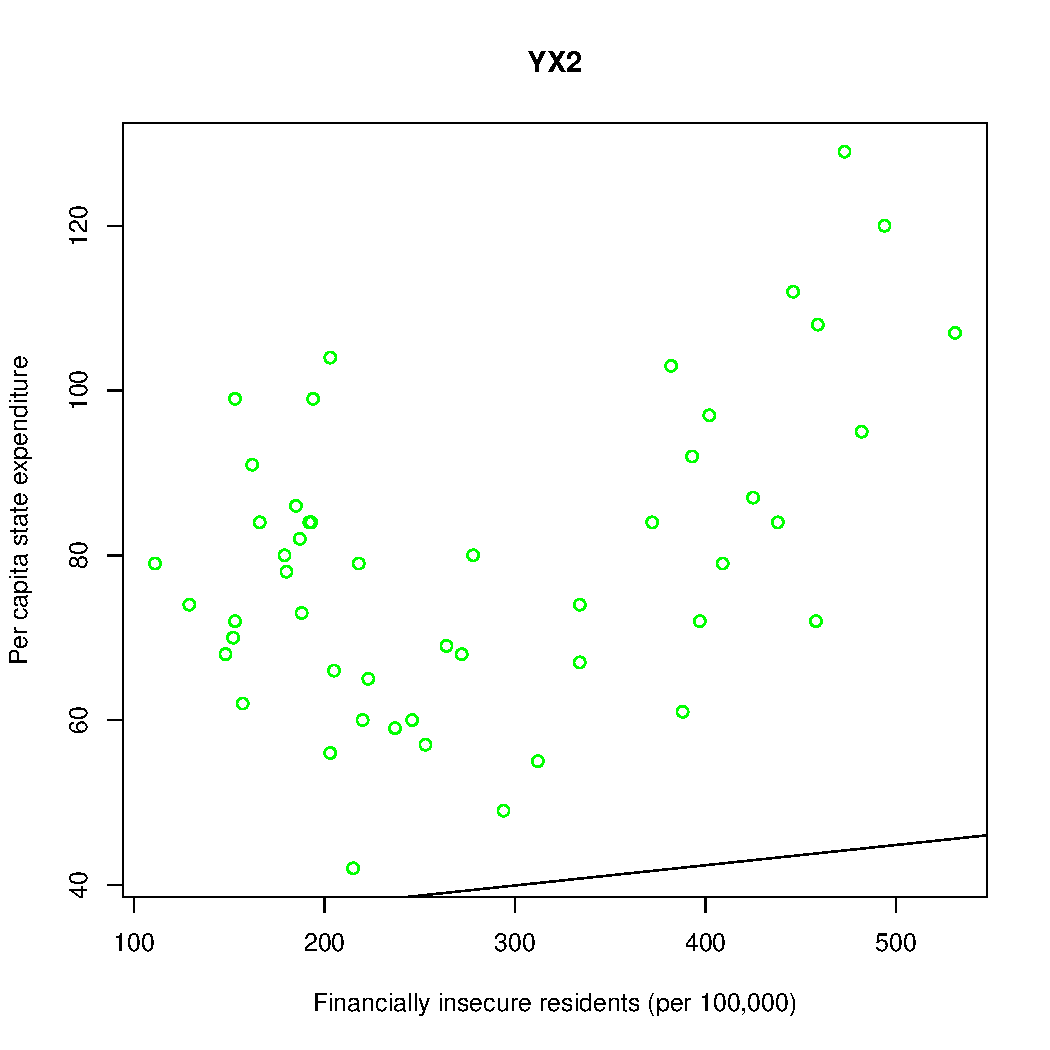
\includegraphics[width=0.7\textwidth]{02.PS01_Skrypnyk_YX2plot.pdf}
\end{figure}


\begin{enumerate}[$\circ$]
	\item The correlation between Per capita expenditure on shelters/housing assistance in state and Number of residents per 100,000 that are "financially insecure" in state follows a (NON-LINEAR) U-SHAPED pattern.
	
	\item \textit {Being honest, this is my first time hearing about a U-shaped relationship, so I searched for the answers \href{https://stats.stackexchange.com/questions/315076/what-is-a-strict-definition-of-u-shaped-relationship}{on the Internet} to understand it:}
	"U-shaped relationship... usually means that the relationship is first decreasing and then increasing, or vice versa. In other words, it means that the relationship is not monotonic (non-monotonic), but instead has exactly one extremum (maximum or minimum)." 
	
	\item From my understanding, there is an initial range where changes in Number of "financially insecure" residents do not have a significant effect on Per capita state expenditure, but starts to increase its effect after a 'turning point' in the bottom of the U-shape.
		\vspace{3cm}

\end{enumerate}

\noindent \begin{center}
	\textbf {\textit{2.1.3:YX3}}
\end{center}

\begin{figure}[H]
	\centering
	\caption{\footnotesize Relationship between Per capita state expenditure and № of Urban residents (per 1000)}
	\label{fig:plot_3}
	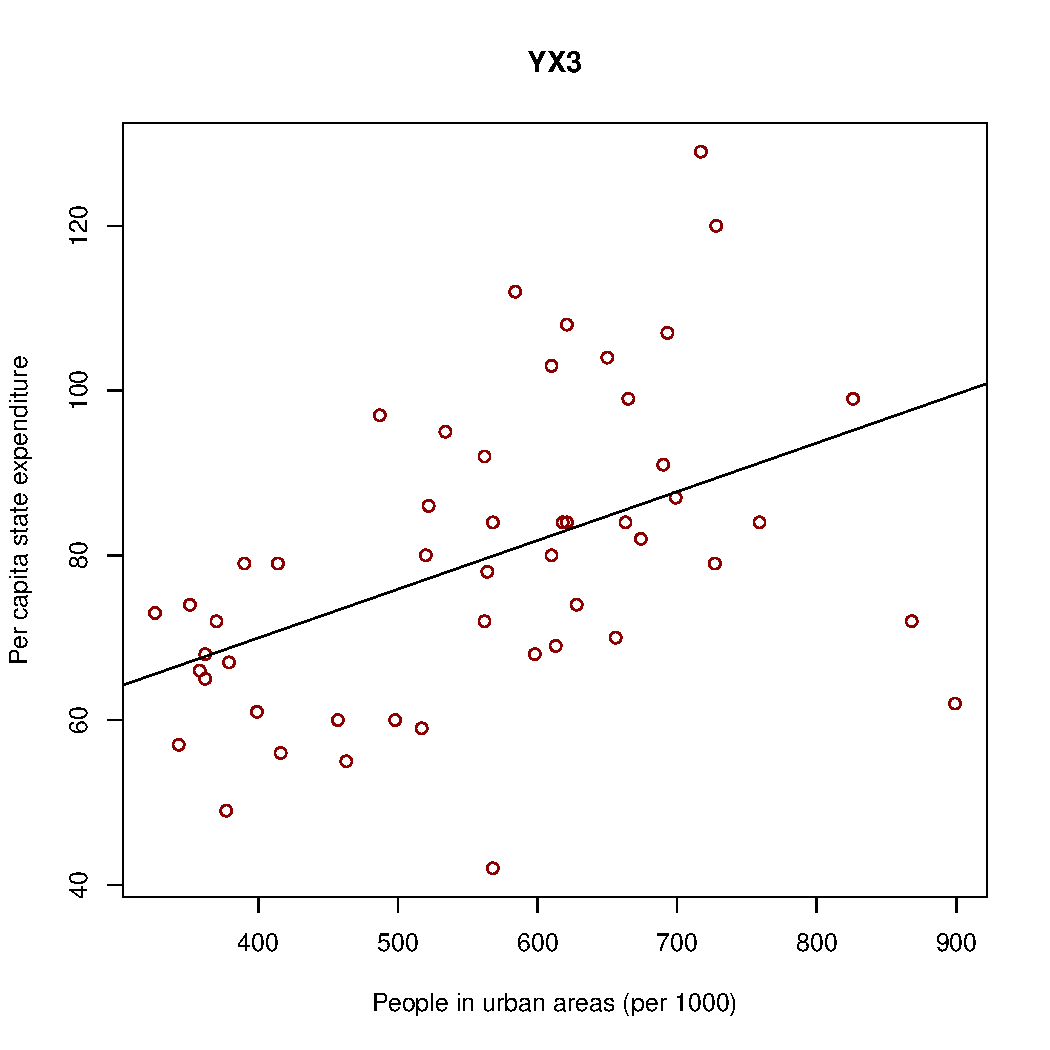
\includegraphics[width=0.7\textwidth]{03.PS01_Skrypnyk_YX3plot.pdf}
\end{figure}

	\noindent 
\centering
\textit{cor = 0.46, positive moderate} 

\begin{enumerate}[$\circ$]
	\item The correlation between Per capita expenditure on shelters/housing assistance in state and Number of people per thousand residing in urban areas in state is LINEAR, POSITIVE, MODERATE (with a few outliers). 
	\item As the Number of urban residents increases, Per capita state expenditure on shelters/HA tends to increase as well, but this correlation is not strong.
	\vspace{5cm}
\end{enumerate}

\noindent \begin{center}
	\textbf {\textit{2.1.4:X1X2}}
\end{center}

\begin{figure}[H]
	\centering
	\caption{\footnotesize Relationship between № of Financially insecure residents in state (per 100,000) and Per capita personal income in state}
	\label{fig:plot_4}
	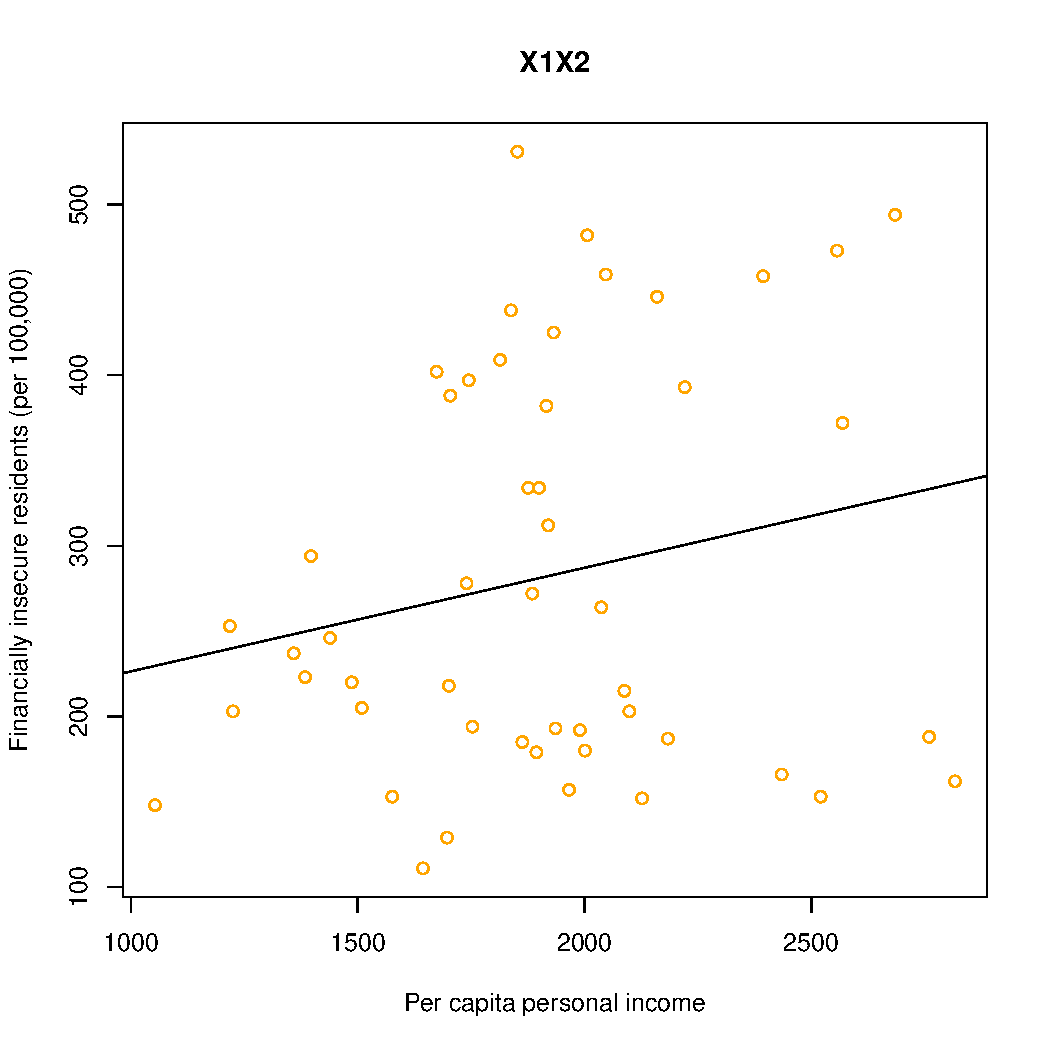
\includegraphics[width=0.7\textwidth]{04.PS01_Skrypnyk_X1X2plot.pdf}
\end{figure}

\noindent 
\centering
\textit{cor = 0.2, positive weak} 

\begin{enumerate}[$\circ$]
	\item The correlation between Per capita personal income in state and Number of residents per 100,000 that are "financially insecure" in state is LINEAR, POSITIVE, WEAK.
	\item As Per capita personal income in state increases, Number of Financially insecure residents in that state tends to decrease, but this tendency is quite weak, and there are probably other factors that influence this variable more strongly. 
	\vspace{5cm}
	
\end{enumerate}

\noindent \begin{center}
	\textbf {\textit{2.1.5:X1X3}}
\end{center}

\begin{figure}[H]
	\centering
	\caption{\footnotesize Relationship between Per capita personal income in state and № of Urban residents (per 1000).}
	\label{fig:plot_5}
	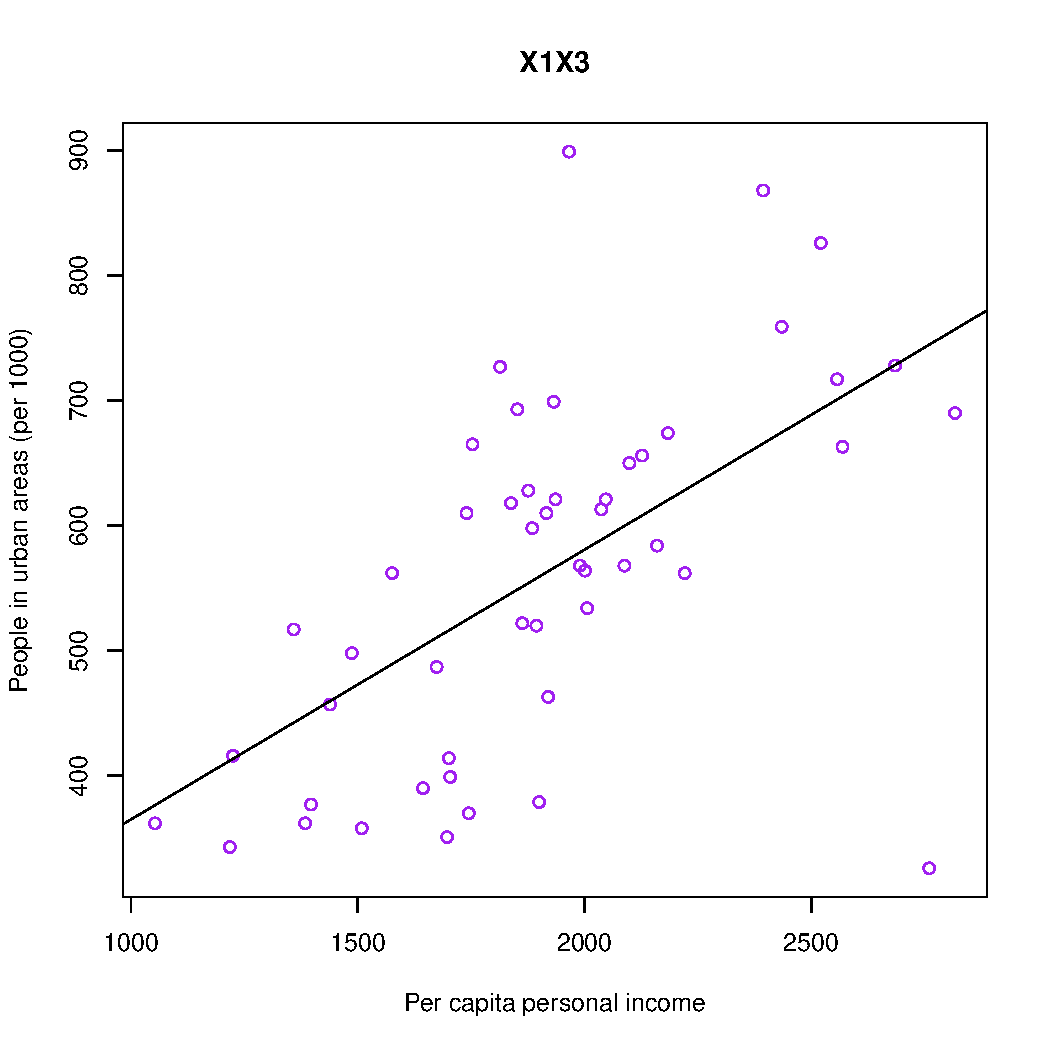
\includegraphics[width=0.7\textwidth]{05.PS01_Skrypnyk_X1X3plot.pdf}
\end{figure}

\noindent 
\centering
\textit{cor = 0.6, positive moderate} 

\begin{enumerate}[$\circ$]
	\item The correlation between Per capita personal income in state and Number of people per thousand residing in urban areas in state is LINEAR, POSITIVE, MODERATE.
	\item As Per capita personal income in state increases, Number of urban dwellers tends to increase as well. However, the correlation is not very strong(though the strongest of all our cases), and other factors' influence may play its role.
	\vspace{5cm}
	
\end{enumerate} 

\noindent \begin{center}
	\textbf {\textit{2.1.6:X2X3}}
\end{center}

\begin{figure}[H]
	\centering
	\caption{\footnotesize Relationship between № of Financially insecure residents in state (per 100,000) and № of Urban residents (per 1000).}
	\label{fig:plot_6}
	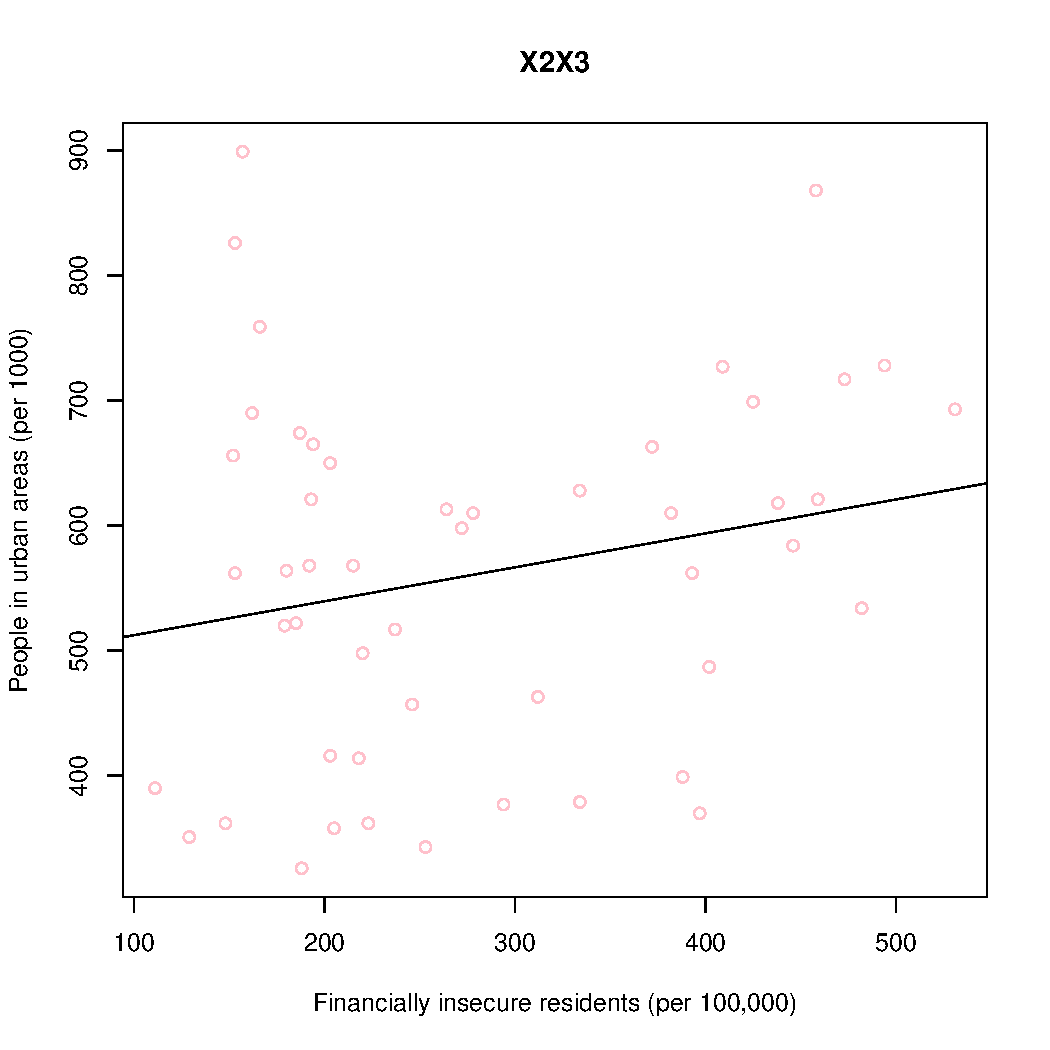
\includegraphics[width=0.7\textwidth]{06.PS01_Skrypnyk_X2X3plot.pdf}
\end{figure}

\noindent 
\centering
\textit{cor = 0.2, positive weak} 

\begin{enumerate}[$\circ$]
	\item The correlation between Number of residents per 100,000 that are "financially insecure" in state and Number of people per thousand  residing in urban areas in state is LINEAR, POSITIVE, WEAK.
	\item As Financial Insecurity increases, Number of Urban dwellers also tends to increase, but this tendency is weak, and there are probably other factors that influence this variable more strongly. 
	\vspace{5cm}
	
\end{enumerate}  

\noindent \begin{center}
	\textbf {\textit{2.1.7: Scatterplot Matrix}}
\end{center}

\begin{figure}[H]
	\centering
	\caption{\footnotesize Scatterplot Matrix (Y, X1, X2, X3)}
	\label{fig:plot_7}
	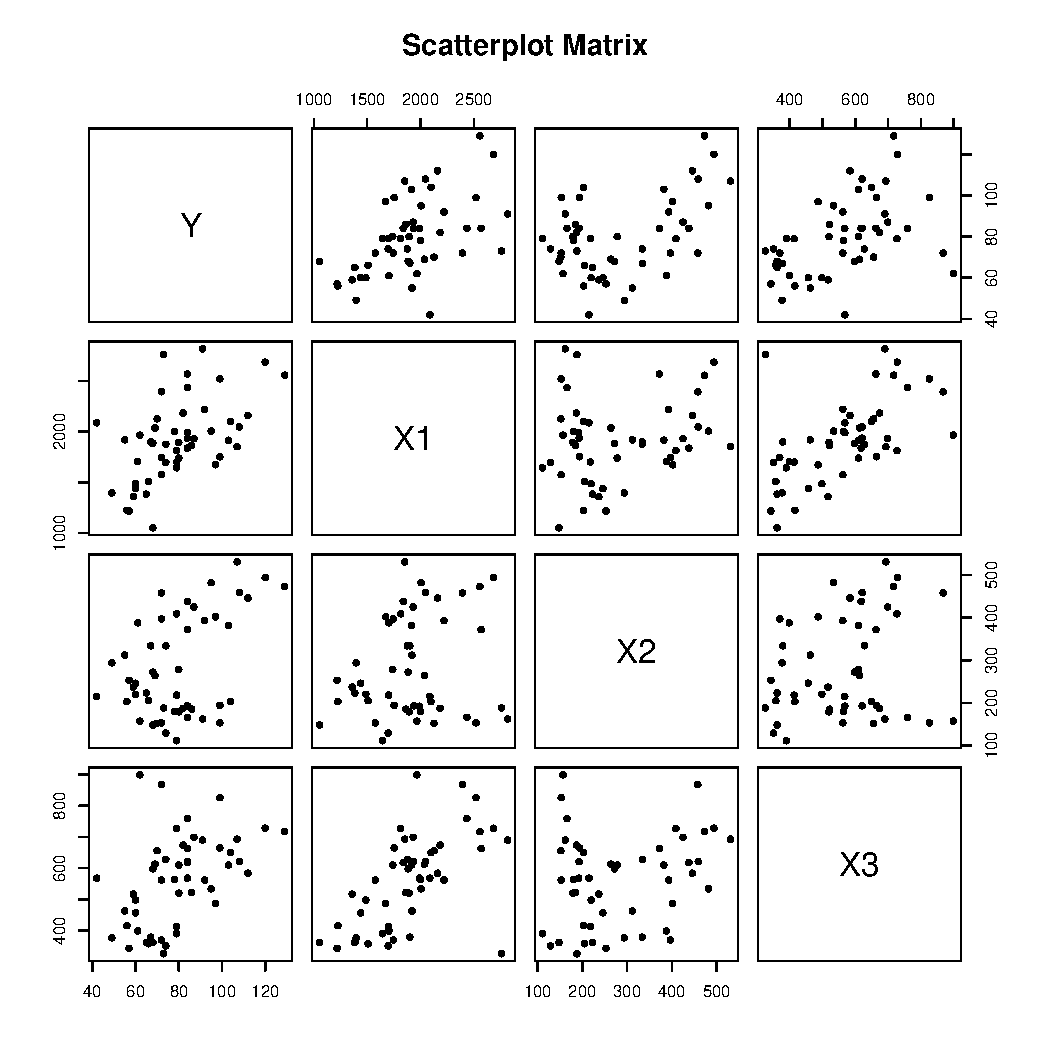
\includegraphics[width=1\textwidth]{07.PS01_Skrypnyk_ScatterplotMatrix.pdf}
\end{figure}

	\vspace{5cm}

\begin{itemize}
\item
\begin{flushleft}
	\textbf {Please plot the relationship between \emph{Y} and \emph{Region}? On average, which region has the highest per capita expenditure on housing assistance?}
\end{flushleft}
\vspace{.5cm}
\end{itemize}

\noindent \begin{center}
	\textbf {\textit{2.2:YRegion}}
\end{center}

\begin{figure}[H]
	\centering
	\caption{\footnotesize Relationship between Per capita expenditure on shelters/housing assistance in state and Region}
	\label{fig:plot_8}
	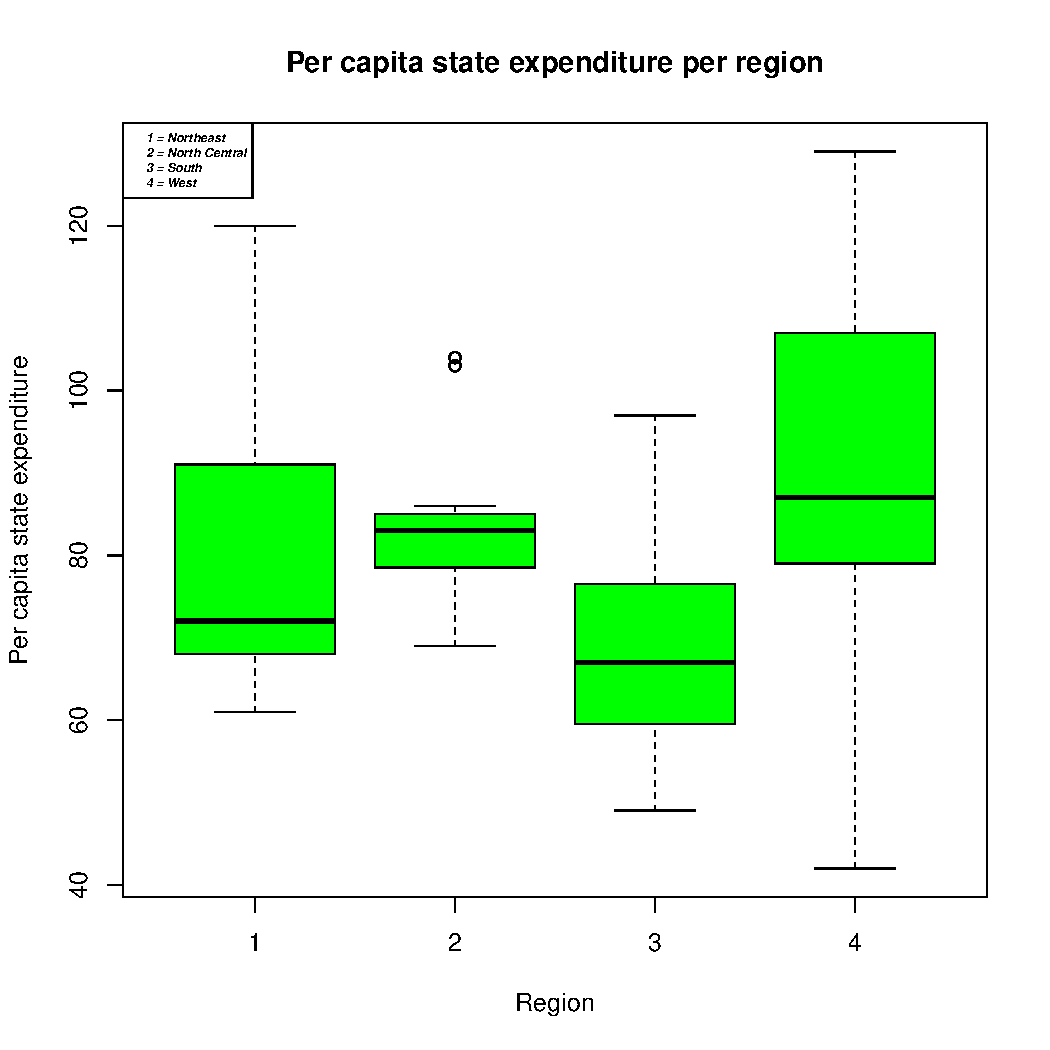
\includegraphics[width=1\textwidth]{08.PS01_Skrypnyk_YRegionplot.pdf}
\end{figure}

\lstinputlisting[language=R, firstline=391, lastline=414]{PS01MS.R}  


	\noindent \begin{flushleft}
		Therefore, REGION 4=WEST, on average, has the highest per capita expenditure on housing assistance (88.30769).
	\end{flushleft}
	\vspace{0.5cm}
	

\begin{itemize}
\item
\begin{flushleft} \textbf 
	{Please plot the relationship between \emph{Y} and \emph{X1}? Describe this graph and the relationship. Reproduce the above graph including one more variable \emph{Region} and display different regions with different types of symbols and colors.}
\end{flushleft}
\end{itemize}

\noindent \begin{center}
	\textbf {\textit{2.3.1:YX1}}
\end{center}

\noindent \begin{center}
	\textit{(Please see the plot on the next page)}
\end{center}

\begin{figure}[H]
	\centering
	\caption{\footnotesize Relationship between Per capita state expenditure and Per capita personal income}
	\label{fig:plot_9}
	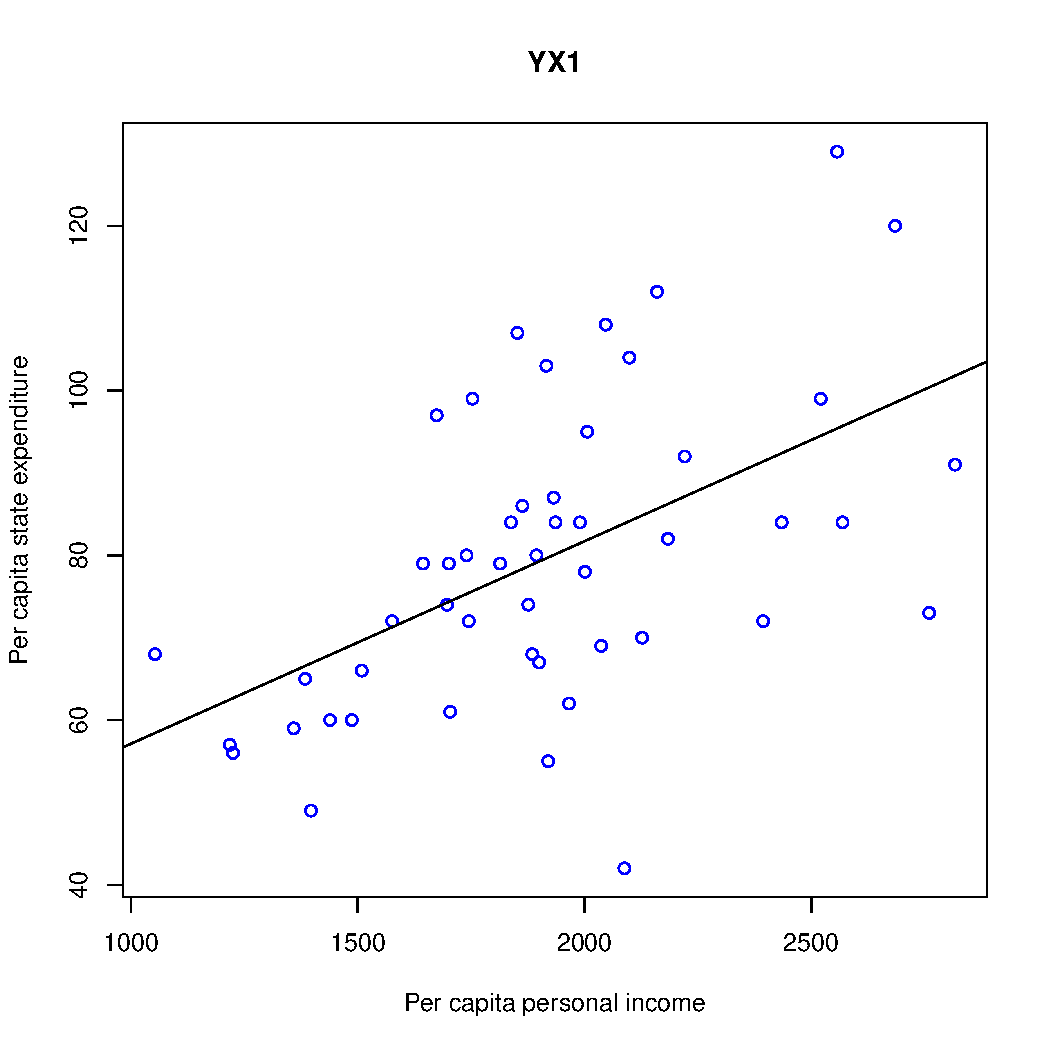
\includegraphics[width=0.7\textwidth]{09.PS01_Skrypnyk_YX1plot.pdf}
\end{figure}

\noindent 
\centering
\textit{cor = 0.5, positive moderate} 

\begin{enumerate}[$\circ$]
	\item The correlation between Per capita expenditure on shelters/housing assistance in state and Per capita personal income in state is LINEAR, POSITIVE, MODERATE (with a few outliers).
	\item As Personal income increases, so does Expenditure on shelters/HA, though this relationship is not strong (+there are exceptions).
	\vspace{5cm}
\end{enumerate}

\noindent \begin{center}
	\textbf {\textit{2.3.2: YX1 by Region}}
\end{center}

\begin{figure}[H]
	\centering
	\caption{\footnotesize Relationship between Per capita state expenditure and Per capita personal income by Region}
	\label{fig:plot_10}
	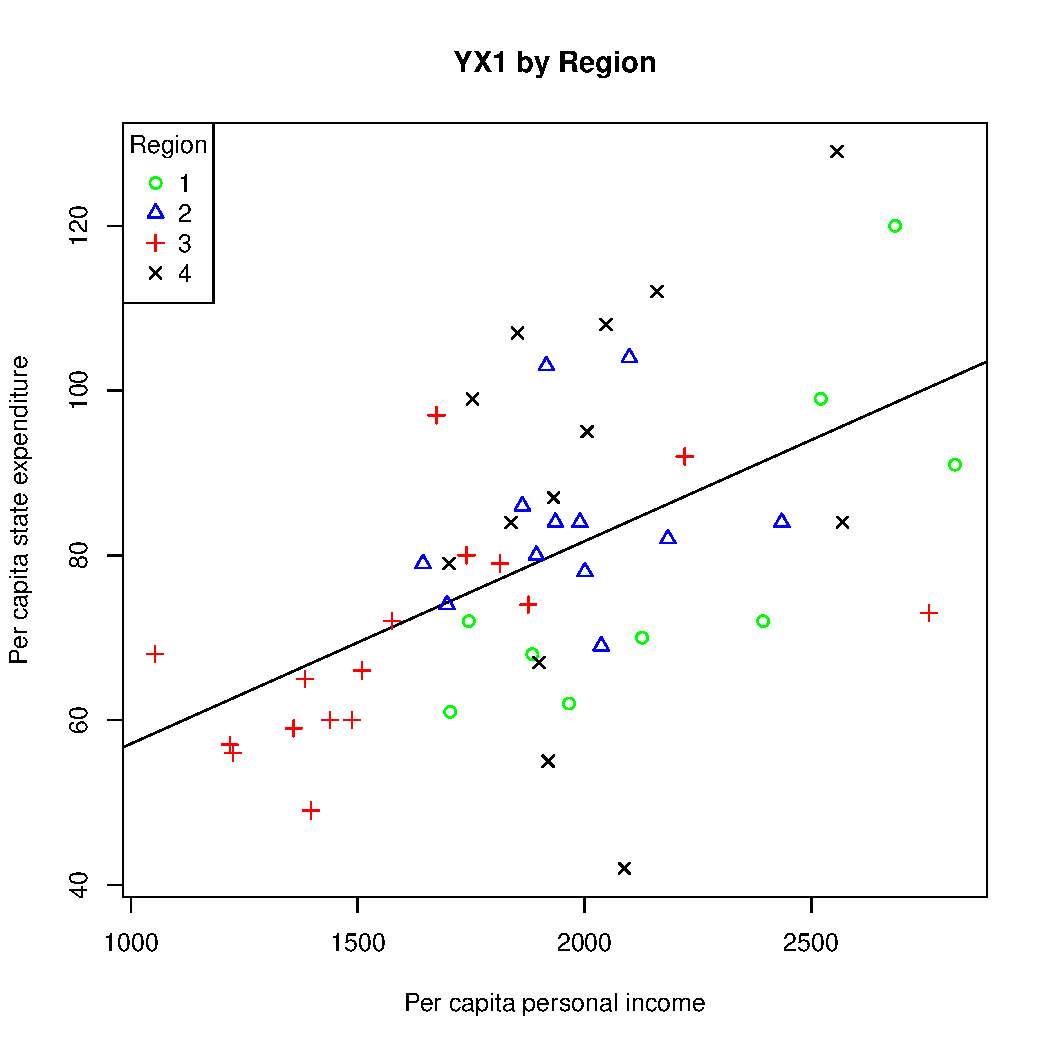
\includegraphics[width=1\textwidth]{10.PS01_Skrypnyk_YX1byRegionplot.pdf}
\end{figure}


\end{document}
